\documentclass[14pt]{article}

\usepackage{geometry}
\usepackage{graphicx}
\usepackage{listings}

\geometry{
	a4paper, 
	top = 2cm,
	left = 1.5 cm,
	right = 1.5 cm,
}

\title{Sistemi Operativi Avanzati}

\begin{document}
\maketitle
\tableofcontents
\section{Blocco 1: Hardware Insights}
Analisi di aspetti che riguardano come i processori sono fatti, come si comportano e come questo impatta sul software in esecuzione. Cominciamo già ad introdurre una serie di problemi per la parte di sicurezza.\\ L'IT si è evoluto dall'Assembly verso B/C, C++, Web API etc... Quindi, astrazioni sempre più lontane da ciò che accade in un sistema, più ci si allontana, più si perdono caratteristiche relative alla parte hardware ovvero dal capire cosa accade quando si scrive qualche applicazione. Si perde anche la capacità di configurazione e la capacità di sviluppare nuove cose, che si scontrano con l'hardware.\\ L'informazione che si perde spostandosi verso l'alto: lo stato del programma è un ecosistema di componenti hardware e software, quando si lavora ad alto livello e si guarda solo il framework specifico è perso. Inoltre, il software oltre a toccare le risorse presenti nell'ISA (registri, memoria etc...), tocca anche lo stato di risorse non nell'ISA: se ho un'istruzione che sposta il dato da un registro ad un altro, lo stato dell'hardware cambia non solo dei registri, ma anche in altro.\\ Ci sono dei footprint lasciati dal software in esecuzione sull'hardware che vanno conosciuti.\\\\ Ci sono sorgenti che, se astratte, si perdono:
\begin{itemize}
\item compiler decision: se non conosciamo le istruzioni usate, perdiamo i side effect
\item hardware run-time decision: tutti gli step che l'hardware esegue per portare avanti un program flow. Quando l'hw esegue le istruzioni, non le esegue sempre allo stesso modo, perché può cambiare lo stato interno. Una delle cose più interessanti è relativo all'hyper-threading: ho dell'hw, unico motore, quanti flussi di istruzioni eseguo? Con l'hyper-threading, più di un flusso quindi bisogna decidere come distribuire la capacità computazionale fra le varie istruzioni. \\ Inoltre, su hw moderno tutte le istruzioni sono eseguite in parallelo, una volta può essere eseguita con i dati in cache ed un'altra no: sono due situazioni diversi.
\item disponibilità dell'hw
\end{itemize}
Ci piacerebbe capire il dettaglio di tutto.\\ Possiamo sfruttare soluzioni già scritte da altri, in quanto sapeva come farlo, ma è utile scendere nel dettaglio. \\\\ 
\subsection{Bakery algorithm di Lamport}
\begin{lstlisting}
var choosing: array[1,n] of boolean;
number: array[1,n] of int;


var choosing: array[1,n] of boolean;
number: array[1,n] of int;
repeat {
	choosing[i] := TRUE;
	number [i] := <max in array number[] + 1>;
	choosing[i] := FALSE;
	for j = 1 to n do {
		while choosing[j] do no-op;
		while number[j] =/= and (number [j],j)< (number [i],i)
		do no-op;
	}
	<critical region>;
	number[i] := 0;
}until FALSE
\end{lstlisting}
posso avere concorrenza reale fra thread, oppure una concorrenza logica. Affrontiamo il problema della sezione critica, si entra a turni e sempre almeno uno è dentro.\\ Per sincronizzare i thread ci sono dei dati condivisi in memoria, due array.\\ Quando un thread vuole entrare, si alza un flag, si sceglie un numero d'ordine (massimo letto +1) e poi si chiude il flag. Occorre aspettare poi il proprio turno, ovvero che i numeri d'ordine non siano stati resettati e confrontando il proprio numero. L'attesa è attiva: è a livello utente, non c'è nessuna chiamata al SO, l'attesa è basata sui numeri ed anche sugli ID dei processi. Facendo girare l'algoritmo sulla propria macchina, ci sono dei problemi dati dall'aver utilizzato un linguaggio come il C senza sapere quale sarà l'hw dove girerà il sw. l'idea è quella di verificare, tramite logging, se il valore del token \textit{tokens\_to\_distribute} viene preso doppio o viene saltato qualche decremento.\\ Il motivo del non funzionamento: \textbf{sequential consitency}, nessuna macchina off the shelf lo è. Quello che succede non è relativo alla compilazione, quindi va in esercizio un programma scorretto, ma l'hardware a run time fa delle cose che non conosco, quindi se questo non viene evitato non è possibile eseguire sw di sistema.\\ Quindi. cominciamo a muoverci per capire cosa accade in hw, ovvero le differenze fra un modello di hw ed il vero hw. Modello:
\begin{itemize}
\item single CPU
\item single memory abstraction
\item single flow control abstraction fatto di fetch, execute e store
\item transizioni di stato nell'hw che sono separate nel tempo: c'è una sola istruzione in flight per ogni istante di tempo
\item immagine definita della memoria allo startup di ogni istruzione
\end{itemize}
Vedendo il processore così, è come se non si eseguisse in parallelo. L'approccio moderno di pensare l'architettura è differente, difatti si considera il concetto di \textbf{scheduling}, cercando di pianificare come fare le cose affinché quello che realmente si fa è \textit{equivalente} che un program flow va a specificare che debba succedere.\\ Abbiamo quindi un program flow, ma non è più vero che quando viene eseguita una istruzione le precedenti hanno impresso l'output come side effect nell'hw, quello che si cerca di fare è mettere in scheduling l'istruzione come se tutto fosse sequenziale (nell'execution flow).\\ Quando poi si astrae dall'hw, si recupera lo scheduling anche a livello sw: un conto è decidere cosa fare del flusso nell'engine, un conto è decidere quali dei molteplici flussi paralleli associare all'engine.\\ È possibile seguire una regola parallela, basta che il program flow non vada diversamente da quanto scritto nel software e quindi c'è la \textbf{propagation of values}, quindi il valore va propagato in avanti per istruzioni successive. Quindi, a livello sw, lo scheduling definisce:
\begin{itemize}
\item la definizione dei time frames per l'esecuzione dei threads sull'hw
\item quando si parla di sw, non si eseguono solo thread, altrimenti il sistema sarebbe sordo rispetto agli interrupt che è un task, quindi serve la definizione dei time frames per servire l'interrupt. Questo non è banale: nel task managment, questo ha portato all'evoluzione smodata nei kernel Linux.
\item Sincronizzazione livello software, ovvero quando i thread devono eseguire le istruzioni macchina in CPU
\end{itemize}
A livello hardware, c'è \textbf{l'istruction based parallelism}: in una finestra temporale in cui una istruzione ha prodotto output, è possibile farne entrare un'altra. Processiamo più istruzioni insieme, che fanno cose differenti. Quindi, ad ogni ciclo di clock è possibile completare le diverse istruzioni una dopo l'altra, quindi completare prima.\\ A livello software c'è il \textbf{thread level parallelism: }ci possono essere più program flow che portano avanti la logica (slides).\\ Su un'architettura ILP non per forza siamo paralleli a livello di thread, ma vale invece il contrario per il parallelismo sw.\\\\ La velocità del processore spesso è misurata come Ghz, ovvero quanto impiega il ciclo di clock a cambiare stato.\\ Sappiamo però che una istruzione entra ad un ciclo di clock ed esce dopo un certo numero di cicli di clock, quindi può usarne un numero elevato, perché fa molte interazioni con l'hw o se ci sono delle asimmetrie o dei pattern di gestione dei dati. Quindi, parlando dei Ghz del processore non stiamo necessariamente parlando di quanto è veloce il processore, conta quali istruzioni usiamo e come queste sono combinate fra loro.\\ Un'altra cosa fondamentale riguarda le categorie di flussi di esecuzione:
\begin{itemize}
\item CPU bound: programma o thread che usa tutto il tempo di CPU a disposizione
\item I/O bound: chiama un servizio bloccante del kernel e quindi usa meno tempo di CPU
\end{itemize}
Esiste una ulteriore categoria di applicazioni, ovvero le \textbf{memory bound:} similari alle CPU bound, ma mentre il program flow del thread è in esercizio, molte delle istruzioni interagiscono con la memoria. Quindi, le istruzioni usano un alto numero di clock perché serve che arrivi qualcosa da qualche componente esterno verso il processore affinché continui l'esecuzione. Questo ha portato allo sviluppo dell'hw in modo da poter sempre fare lavoro utile anche se ci sono istruzioni bloccate nella CPU $\rightarrow$ ILP spinto a livello quasi estremi.\\ Questo ha portato alla ri-progettazione di vari processori, il problema è che l'accelerazione dei processori ha creato un gap fra memoria e processori, problema delle architetture moderne.
\subsection{Pipeline}
Una pipeline fa ILP, in quanto c'è overlap in processing di più istruzioni: una istruzione inizia, mentre questa fa qualcosa ce n'è un'altra che fa qualcos'altro. C'è anche lo scheduling nella pipeline: c'è parallelismo, ma la sequenza delle istruzioni di un program flow non è eseguita necessariamente secondo la stessa sequenza del programma. Bisogna ovviamente mantenere la \textbf{causalità}, altrimenti l'architettura hw non può portare avanti il program flow. Quindi, l'architettura è un data flow model, con il vincolo della causalità (nel flusso di programma) alla base della costruzione di tutte le architetture moderne. Quindi, una architettura moderna implementa un data flow model: ogni istruzione che vediamo in realtà sta avvenendo in parallelo con molte altre, sia in lettura che in scrittura.\\ In una architettura pipeline semplice, una istruzione passa per fasi differenti ed usa nelle differenti fasi componenti diverse del processore
\begin{figure}[ht!]
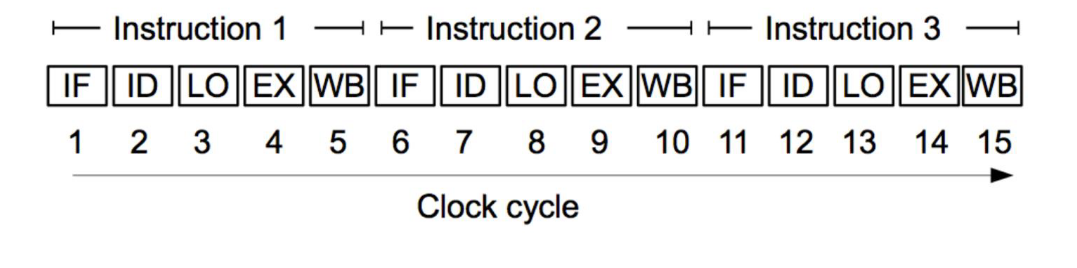
\includegraphics[scale=0.3]{immagini/no-pipeline}
\caption{Istruzioni senza pipeline}
\end{figure}
L'esecuzione in pipeline si basa sulla possibilità di sovrapporre le istruzioni, perché una istruzione non sta usando alcuni componenti della CPU che possono essere usate da altre
\begin{figure}[ht!]
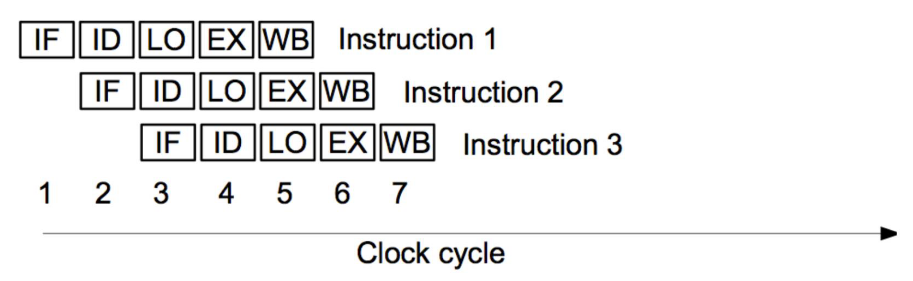
\includegraphics[scale=0.3]{immagini/pipeline}
\caption{Istruzioni con pipeline}
\end{figure}
Questo è l'ILP, e questo tipo di architettura è la base che, con altre tecniche, permettono di eseguire altro per affrontare problemi come il fatto che ogni operazione come la LO richieda più cicli di clock. Non sappiamo quanti cicli di clock richiede una istruzione, quindi il problema va affrontato. Inoltre, l'altro problema è legato ai \textbf{breaks:}se ho un'istruzione di salto e riesco a capire dove saltare solo quando l'istruzione è finalizzata, l'istruzione da mettere potrebbe essere differente da quella da immettere effettivamente e che si saprebbe solo alla fine. Questo è il problema della \textbf{control dependency}, altro problema è la \textbf{data dependecy}, dove il dato è richiesto da una istruzione in un momento in cui non è disponibile.\\ Analisi di cosa vuol dire usare pipeline: (vedi slides). Ovviamente, abbiamo uno speed up ideale, il problema è che non consideriamo i problemi sopra citati: non è detto che si riesce a committare una istruzione per ogni ciclo di clock, quindi possono essere richiesti molti più cicli di clock. Ampliando la pipeline, si amplia la \textbf{capacità di fare}, quindi inserire nel processore hw per fare operazioni che poi magari non vengono eseguite.
\subsection{Processori moderni}
Gli stage di pipeline non è molto elevato, quindi vediamo come è stato sfruttato per risolvere tutta la serie di problemi visti.\\ Abbiamo:
\begin{itemize}
\item software stall: inseriamo in un flusso di programma delle istruzioni di stallo fra due istruzioni. Se ho un salto e non so dove, metto degli stalli finché so se saltare o meno
\item software re-sequencing: fatto dai compilatori, quando si rendono conto che un blocco atomico di programma (ovvero un flusso eseguito tutto) si ri-organizza il blocco di istruzioni in modo che istruzioni che si dipendono siano più distanziate
\item per i salti, c'è la branch prediction: se non si sa quale è l'istruzione, si fa una previsione e si fa il fetch di quella zona di codice
\item out-of-order pipeline (OOO): la base di ciò che accade in una architettura moderna. Importantissimo per permettere alla CPU di essere efficace ed efficiente con generiche sequenza di istruzioni: se una istruzione deve aspettare dei dati, un'altra successiva può andare avanti ed anche completare \textbf{ma senza rendere visibili le cose nell'ISA}, o si viola il flusso di programma. Quindi, l'OOO non è basato su come le istruzioni toccano l'ISA, ma sul fatto che alcune istruzioni devono aspettare.
\end{itemize}
\subsection{Concetti base di x86}
Il processore x86 a 64 bit moderno ha più o meno lo stesso set di registri di un processore x86, la differenza è che sono un po' di più e sono più grandi.\\ I cambiamenti sono all'interno, ovvero come vengono eseguite le istruzioni: i486 è stato il primo ad adottare una architettura pipeline, riportata in seguito
\begin{figure}[ht!]
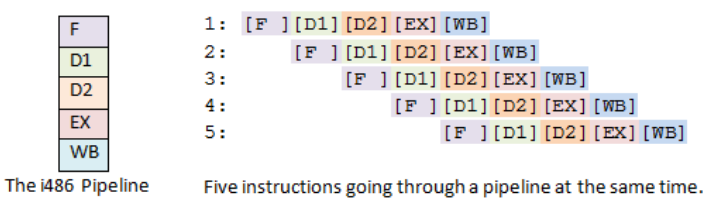
\includegraphics[scale=0.4]{immagini/pipeline-i486}
\caption{Pipeline di i468}
\end{figure}
L'architettura non è "piaciuta" molto, ad esempio per fare uno swap fra due registri questo richie 3 istruzioni, ma facendo diversi XOR ognuno dipende dal precedente, e questo rallentava tutta la pipeline.\\ Se ad esempio, abbiamo del codice C che accede ad un puntatore ed in un caso accede e poi incrementa il puntatore, oppure se accede dopo aver incrementato ha un effetto totalmente diverso. È possibile sperimentare lo stesso problema anche in linguaggi di più alto livello, ad esempio se si incrementa un puntatore:
\begin{itemize}
\item a = *++p
\item a = *p++
\end{itemize}
c'è una differenza in performance evidente fra i due statement.\\ C'è inoltre il problema di istruzioni che causano lo sqash della pipeline, ovvero viene cancellato tutto ciò che è contenuto nella pipeline. Tali istruzioni possono essere denotate come danno nel nostro programma, in quanto è possibile che vada rifatto il valore cancellato dalla pipe. Se consideriamo x86, una istruzione di questo tipo è \textsf{CPUID}, che prende l'ID numerico del processore su cui si sta lavorando. Questo è fondamentale quando si scrive del sw per il kernel, specialmente quando si sta scrivendo del sw che tocca delle strutture dati per lo specifico processore: bisogna conoscere quale è il processore su cui si lavora.\\ Tali istruzioni sono dette \textbf{serializing}, se però leggiamo il manuale dell'istruzione CPUID ci dice che è garantito che tutto ciò che viene fatto prima è stato completato prima che la prossima istruzione sia fetchata.
\subsection{Intel x86 superscalar pipeline}
Per superare il problema degli effetti del sw all'interno dell'esecuzione della pipeline richiede una  pipeline avanzata per capire cosa è possibile eseguire in parallelo etc: \textbf{superscalar pipeline}. Tale pipeline è fatta in modo che in ogni fase c'è più di un componente, ad esempio più componenti di esecuzione che possono essere identici e l'istruzione può andare in uno di essi. Se ad esempio l'istruzione richiede l'engine per più cicli di clock, non blocca successive istruzioni che magari poi richiedono lo stesso componente. C'è quindi parallelismo nella pipepline stessa, inoltre c'erano anche caratteristiche che faceva si che se c'era parallelismo e una istruzione stava passando avanti usando un'altra istanza del componente è che ciò che accade nella reale implementazione è che questa era basata su out-of-order: se qualche istruzione è ferma, le altre vanno avanti rispettando comunque il data flow model.\\ Tali aspetti erano nati molto prima, ad esempio nell'IBM 360/91 degli anni 60', si parlava però di architetture particolari.\\ Il tutto preveda che nella pipeline ci fossero altri componenti per gestire l'OOO.\\ Le basi del progetto erano:
\begin{itemize}
\item come mettere in commit le istruzioni in program order: fare uscire una istruzione dalla pipe indica che l'effetto dell'istruzione sulle risorse dell'ISA sono visibili, quindi è delicato capire quando mandare in commit
\item processare istruzioni indipendenti, sia sui dati che sulle risorse, il prima possibile
\end{itemize}
Il processore moderno ha una esecuzione differente da quello che accade in teoria nella pipeline: lo scenario in figura 1 è simulato, ma non è quello reale.\\ Vediamo come affrontare il problema che ogni istruzione possa durare un certo numero di cicli di clock
\subsubsection{Istruction span problem}
Ogni istruzione può durare un certo numero di clock, a seconda di cosa deve fare e per effetti diversi, ad esempio che occorre attendere componenti esterni alla CPU come la memoria. Il fetch dei dati può portare via diversi cicli di clock, e si è cercato di risolvere questo come problema centrale con le pipeline superscalari.\\ Con una OOO pipeline, può accadere la seguente cosa\\\\
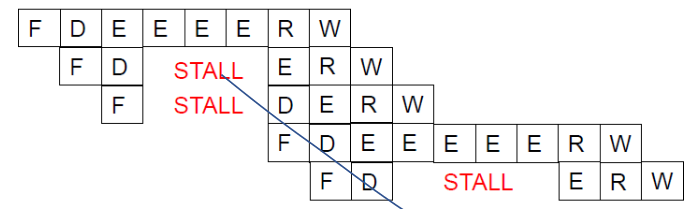
\includegraphics[scale=0.5]{immagini/ooo-pipeline-1}\\
può accadere che la seconda istruzione abbia uno stallo, magari perché non ha i dati. Come vediamo, in realtà l'istruzione ha bisogno di un solo ciclo di clock di esecuzione, ma ne usa di più perché non ha i dati disponibili. Anche la 3° istruzione è bloccata e lo stesso vale per l'ultima, perché deve usare lo stesso componente. Ricordiamo che il delay può avvenire perché il componente da usare non è pronto.\\ In OOO accade la seguente cosa:\\\\
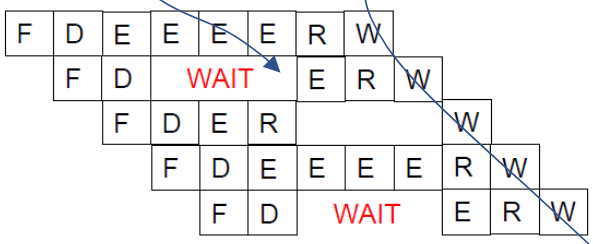
\includegraphics[scale=0.5]{immagini/ooo-pipeline-2}\\
può accadere che istruzione 1 e 2 usano due componenti identici nella pipeline, e 3 entra in esecuzione ed ha pronto il risultato molti cicli di clock prima di quando serve, quindi occorre mantenerla uncommitted e metterla in write back solo in maniera coordinata. Ad ogni ciclo di clock è possibile mandare in commitment il lavoro anticipato: se riusciamo a far entrare una istruzione ogni ciclo di clock, riusciamo a farne uscire una ogni ciclo di clock, avendo lo stesso throughput in ingesso ed in uscita rispetto alla pipeline tradizionale.
\subsection{Pipeline OOO speculativa}
Quando si parla di pipeline OOO, si parla anche di pipeline speculative: su un flusso di programma, se processiamo una istruzione successiva rispetto ad una che deve ancora essere processata, stiamo dicendo che c'è indipendenza fra le due, ma questo non è sempre vero. Quello che è in pipeline sta eseguendo in maniera speculativa, si fa fetch e poi magari le istruzioni non verranno eseguite perché si salta altrove. Inoltre, una istruzione in qualunque ciclo di clock può generare una trap: si potrebbe consultare il TLB (caching), ci rendiamo conto che qualcosa non va e quindi l'istruzione non può essere mandata in commit. Se c'è una trap mentre un program flow esegue, va passato il controllo ad un gestore lato sw, quindi tutte le istruzioni che venivano eseguite dopo erano eseguite in maniera speculativa.\\ Il \textbf{retire} è l'azione del committare una istruzione a rendere i cambiamenti "visibili" in termini di ISA, mentre l'\textbf{emissione} è l'azione di iniettare le istruzioni nella pipeline. Fra le due è possibile che ci siano altre istruzioni, ci sono poi anche le eccezioni che vanno gestite correttamente: se una istruzione entrata in pipeline genera una eccezione, ha senso eseguire un cambio di flusso per gestire l'evento particolare? No, in quanto l'istruzione è eseguita in modo speculativo. Finché non arriva alla fare di write back, questa può scomparire dal flusso, perché anche le istruzioni precedenti sono speculative e magari una istruzione precedente genera l'eccezione che rende l'eccezione di quella successiva inutile, perché l'istruzione non doveva proprio essere nel flusso di programma.\\ Quindi le eccezioni sono imprecise, non è detto che quando vengano generate queste esistano o meno, lo saranno solo se le istruzioni arriveranno al commit point.\\ Inoltre, l'eccezione viene generata considerando che in parallelo stiamo facendo altro in una OOO pipeline:
\begin{itemize}
\item una istruzione precedente è stata superata
\item una istruzione successiva ha superato
\end{itemize}
quindi quando viene generata la trap, lo stato effettivo del processore e quindi di tutti i componenti non esposti nell'ISA, globalmente può essere stato cambiato parzialmente da istruzioni che precedevano quella che ha generato la trap ma anche da istruzioni successive. Quindi, tutte queste istruzioni possono generare dei side effect, che possono essere sfruttati per attaccare le applicazioni ed i sistemi, prelevare dati a cui non si può accedere etc...\\ Di seguito, viene mostrato uno schema esemplificativo della pipeline OOO\\\\
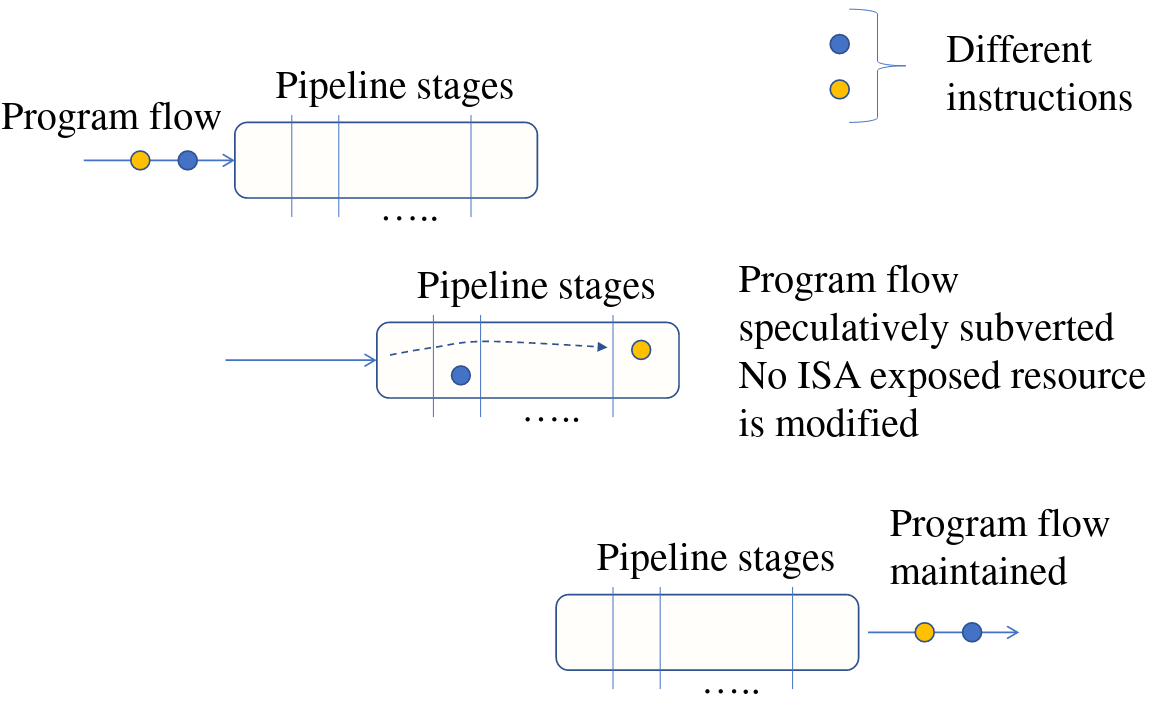
\includegraphics[scale=0.2]{immagini/pipeline-ooo}\\
può accadere che l'istruzione gialla arrivi prima a commit poi di quella blu, e questo permette di portare a termine lavoro utile anche quando altre istruzioni sono bloccate per i vari motivi detti prima.
\subsubsection{Eccezioni imprecise}
Su una architettura pipeline OOO (ma anche generale) in cui le istruzioni si superano l'un l'altra con un ILP molto elevato, consideriamo che una istruzione A è dopo una B nel program flow e B causa una eccezione. Quindi, B $\rightarrow$ A (B precede A), A entra in pipeline prima di B. Se B ha una eccezione, possono esserci tante altre istruzioni successive in pipeline e queste possono aver cambiato molto nello stato della CPU, tutte le relazioni di dipendenza possono essere portate avanti in maniera speculativa senza toccare i registri di CPU, ma toccando altri elementi. Può accadere che ci siano anche altre relazioni, ad esempio B genera dei valori che poi verranno usati da A e che A poi passi il risultato ad altre dopo etc... Si toccano componenti nella CPU in funzione del fatto che vengono anche passate informazioni in maniera speculativa e non a livello dell'ISA. Questo è stata la base dell'attacco meltdown, in cui è stata necessaria la patch di tutti i kernel esistenti: è possibile usare i processori OOO per leggere dati del kernel, è possibile leggere buffer cache e quindi leggere i file o i metadati per proteggere i dati (ad esempio dati di cifratura).
\subsection{Schema}
Quindi, se siamo in pipeline occorre stare attenti, altrimenti si scrive software di sistema non corretto. Può accadere che viene passato un output in maniera speculativa e che ci siano effetti su altri componenti della CPU. Vediamo dei dettagli su come è fatta una pipeline internamente.
\subsubsection{Algoritmo di Robert Tomaluso}
Le architetture moderne hanno delle varianti rispetto a questi algoritmi. Consideriamo come avviene il passaggio fra due istruzioni A e B per cui A$\rightarrow$B nel program flow, queste sono date perché:
\begin{itemize}
\item RAW (Read After Write): B legge dei dati prima che A li scriva, che porta ad uno stallo, dipendenza sui dati
\item WAW (Write After Write): B scrive dei dati prima A scriva lo stesso dato. Il dato espone un valore di stallo
\item WAR (Write After Read): B scrive un dato prima che A legga lo stesso dato, quindi il dato letto non è consistente.
\end{itemize}
Come risolviamo queste dipendenze sui dati: Tomasulo propone delle idee algoritmiche, per un processore OOO:
\begin{itemize}
\item RAW: per ciascuna lettura, bisogna tenere conto se il valore da leggere è già stato prodotto. Occorre quindi tenere traccia del fatto che il dato sia già stato prodotto, l'attesa del dato va quindi inserita nella OOO, quindi considerare il buffering dell'operazione
\item WAR e WAW: soluzione dei \textbf{renamed register}. Supponiamo di avere un registro R, per gestire WAw facciamo si che i due valori siano scritti ma sue due registri diversi. R non è un singolo registro, bensì è un multi-registro, dove ci sono varie versioni del dato. Qualsiasi istruzione deve scrivere un valore in un registro ed entra in pipeline va sul componente, preleva uno slot utilizzabile e scrive il valore in quello slot. Quindi, nel program flow può accadere che i valori possono essere scritti in tempi differenti sullo stesso registro, si risolve quindi WAW che si avrà in termini di commit del valore. Il valore non può sovrascrivere, perché viene scritto su uno slot, quando viene mandato in commit l'istruzione si avrà il valore effettivo associato al registro R, nel controller del registro c'è anche quale è la versione attuale del valore del registro.\\ Un solo valore alla volta è quello attivo, alcune versioni saranno del passato ed altre del futuro, nella storia dei commit che poi verrà realizzata.\\\\
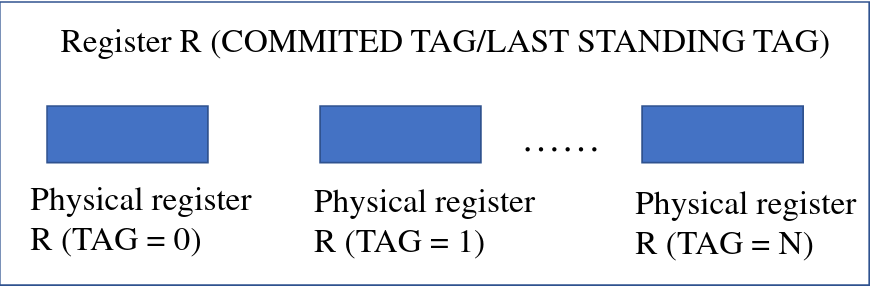
\includegraphics[scale=0.25]{immagini/multi-registri}\\
Quindi, quando mandiamo in pipeline una istruzione che deve leggere R, la marchiamo con il valore che quella deve leggere e finché il registro non è pronto l'istruzione rimane bloccata. Tutto questo è invisibili al programmatore in termini di risorsa ISA, ma visibile in termini del fatto che è possibile far si che il software faccia cambiare stato a tutti i registri in modo da creare problematiche.\\ In maniera indiretta è stato risolto anche WAR: per WAW è stato risolto il problema utilizzando i tag, ma anche per WAR finché il tag da leggere non è pronto, l'istruzione rimane ferma
\end{itemize}
\paragraph{Reservation stations}
Ogni istruzione ha un codice operativo, che va bufferizzato da qualche parte e poi va relazionato al componente che deve eseguire l'operazione. La reservation station è una zona del processore in cui viene registrata una operazione in input all'oggetto che può eseguire quella operazione, ad esempio somme etc... ai componenti corretti, ovvero che possono processarle. Non è detto che l'operazione venga processata immediatamente, perché può essere coinvolta in una dipendenza e dover attendere dei dati non ancora prodotti; questo viene detto dallo stato del renamed register. La reservation station riserva la possibilità di riservare il componente, finché l'istruzione non è pronta ad essere eseguita.
\paragraph{CDB e ROB}
Supponiamo di avere una reservation station in cui ci sia una operazione in coda: il flusso di informazioni fra le componenti deve essere supportato, che avviene usando il Common Data Bus, che permette di spostarle fra i vari componenti per permettere il corretto flusso di input fra le varie istruzioni.\\ C'è anche il Re Order Buffer: bisogna ricordarsi quale è l'ordine logico con cui andare a committare le operazioni, questo tiene conto dell'ordine. Viene gestito circolarmente e ogni slot viene liberato nel momento in cui viene committata l'operazione.
\\\\
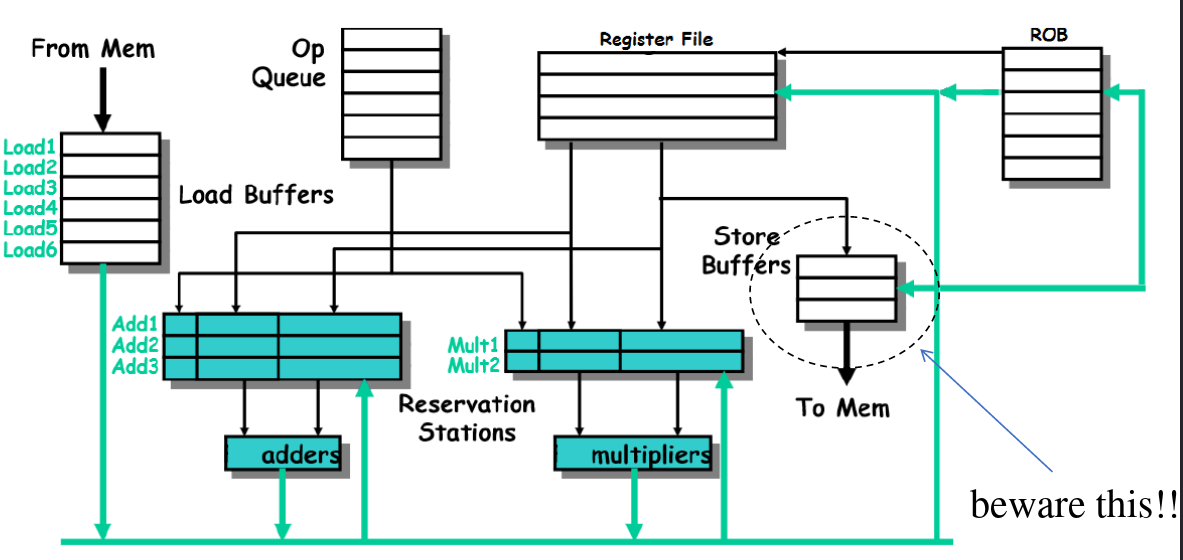
\includegraphics[scale=0.25]{immagini/arch-moderna}\\
Lo store buffer è un altro componente interessante: è fondamentale per interagire con la memoria. Mantiene in maniera temporanea il valore da scrivere per i dati verso la memoria. Lo SB viene toccato solo quando viene committata una istruzione, ed il valore viene scritto nello SB, non in memoria: in una architettura OOO quindi non si ottimizza solo il pipelining, ma anche la scrittura verso la memoria, perché se dovessimo scrivere in memoria a commit-time, la entry del ROB sarebbe occupata per vari cicli di clock e bloccherei diversi componenti senza poter andare avanti. Dallo SB i valori possono anche essere letti, e finché il valore non viene riportano in memoria è visto solo dal singolo program flow. Questo è il problema della sequential consistency, dove se qualcuno produce qualcosa questo non è visibile ad altri.\\\\ \textbf{esempio:} abbiamo 3 istruzioni che entrano in pipeline, con i rispettivi delay $\delta$ per essere processate.
\\\\
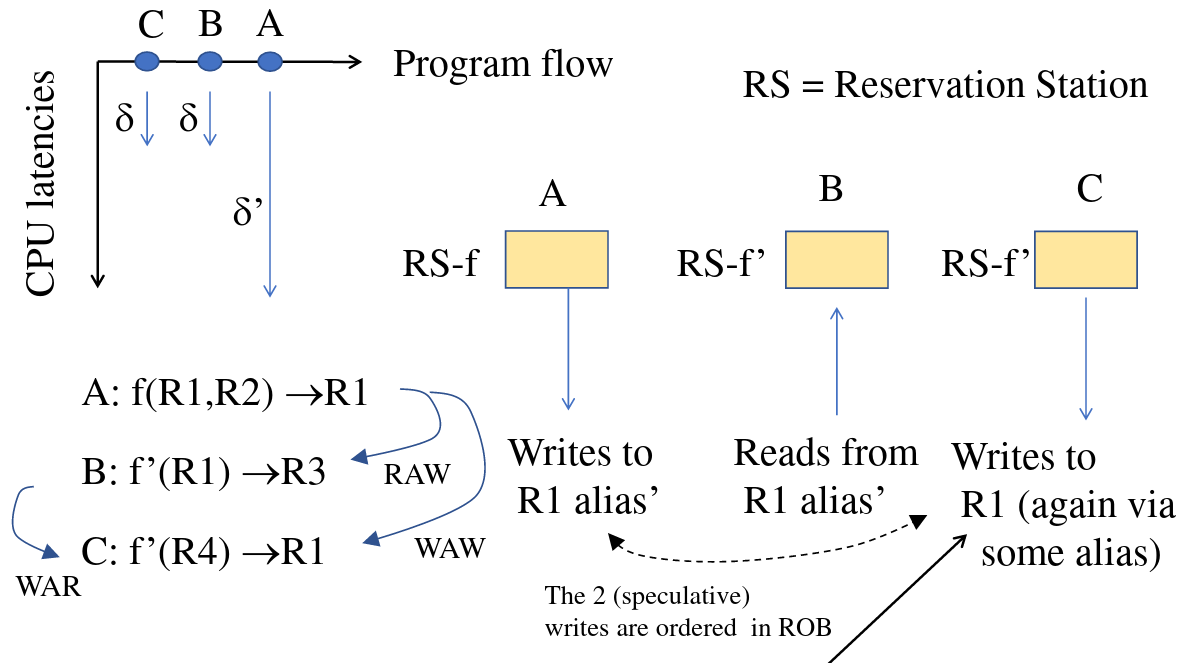
\includegraphics[scale=0.25]{immagini/ex-pipeline}\\
Questo è ciò che avviene realmente quando si esegue in pipeline di questo tipo istruzioni 
%slide dove fa vedere cosa accade
\subsubsection{Storia}
L'architettura basata sull'algoritmo di Tomasulo venivano mandate out of order solo determinate istruzioni, nei processori moderni l'OOO è visibile su tutto l'insieme delle istruzioni. Nell'evoluzione storica c'erano solo istruzioni in floating point, oggi si copre tutto il set di istruzioni
\subsection{Ancora sulla memoria}
Nel tempo, la memoria ha accelerato nella capacità di fornire informazioni, ma i processori hanno accelerato ancora di più nella richiesta delle chiamate a memoria. Quindi, guardando le 3 istruzioni precedenti ed i delay, ci sono anche i delay dovuti alla latenza per i miss in cache. Come vedremo, questo è stato il motivo della nascita delle architetture hyper-threading, ovvero la divergenza fra i due mondi.
\subsection{OOO nell'x86}
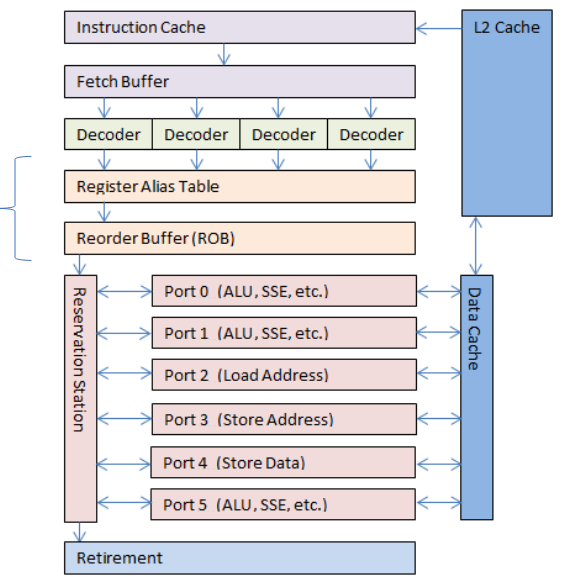
\includegraphics[scale=0.3]{immagini/x86-ooo}\\\\
A livello alto, nell'x86 abbiamo la Register Alias Table, il Reorder Buffer e tutta una serie di hardware replicato. Quando un oggetto entra nel Reorded Buffer, il firmware sceglie uno o l'altro componente replicato; ci sono poi le diverse relazioni che esistono fra i diversi componenti.\\ Questo fa capire che le istruzioni vengono caricate più alla volta, viene caricata una linea di cache che in 86 è da 64 byte, in cui si possono mettere diverse istruzioni, alcune andranno in commit ed altre no, però ci sono molte cose che si passano informazioni e fanno attività.
\subsubsection{Hyperthreading}
La necessità della nascita delle architetture hyper-threading è nata perché la struttura della CPU era talmente ottimizzata da rimanere senza fare nulla per troppo tempo, non riusciva più ad essere fillato in maniera efficiente quando i dati dovevano salire in memoria.\\ Le architetture ad hyper-thread prevedono che, siccome il "motore" è così rapido ed efficiente, si mandano due linee di input in parallelo, che sono due processori effettivi su un unico core: due program flow diversi su i due processori. Quando poi le istruzioni sono processate, si usa l'unico engine: il classico è avere 2-1 (es: 8 thread, 4 core). C'è una buona replicazione dei componenti, per evitare che se un flusso insista su un componente in particolare, non ci sia blocco.\\ Altro aspetto di sicurezza: c'è un interferenza fra i due thread in esecuzione che prevede che si vedano dati da uno all'altro, quindi bisogna "spegnere" uno dei due e sfruttare meno potenza effettiva.
\\\\
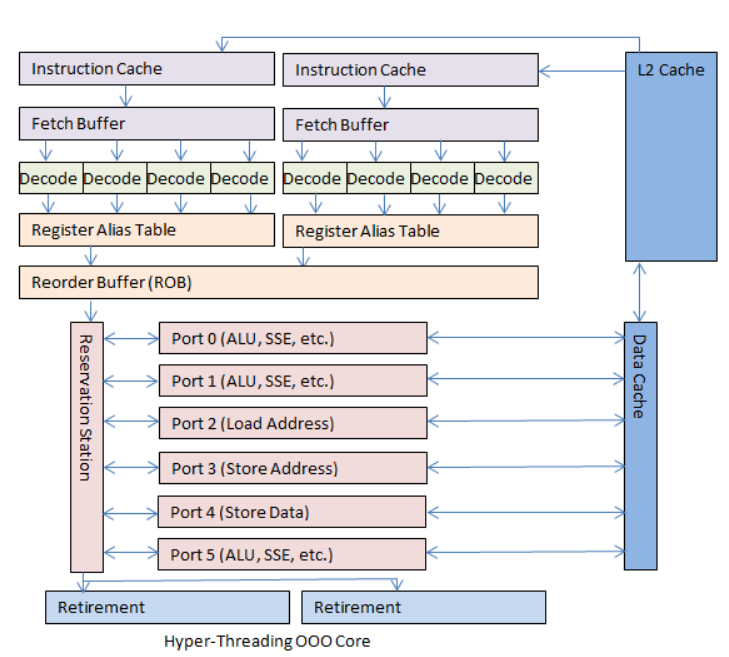
\includegraphics[scale=0.3]{immagini/hypert-ooo}\\
In questa architettura ci sono due hyper-thread ed una sola architettura per processare le istruzioni dei flussi e non c'è interferenza fra i due flussi, quindi quando l'istruzione scrive su un registro la risorsa è accessibile solo da quel flusso, ma la scrittura è tale per cui i componenti siano utilizzati per le istruzioni anche dell'altro flusso ma queste vengono usate in time sharing: gli oggetti non sono esposti nell'ISA, quindi questo non crea problemi a cosa è scritto nei programmi. In ogni caso, ci sono dei side effects sugli engine quando si esegue in hyper-threading, che sono problematici per la sicurezza.
\subsection{Gestione degli interrupt}
Ogni sistema moderno è interrupt-driven, quando c'è un interrupt bisogna eseguire una porzione di codice per rispondere agli interrupt.\\ Quando siamo sulla pipeline, avere un interrupt significa dire che siamo entrati con una serie di istruzioni sul thread corrente e l'interrupt vuole che si passi a prelevare istruzioni da un'altra zona di memoria, l'interrupt si accetta sempre quando una istruzione ha completato (per evitare di dover salvare lo stato dell'istruzione corrente). Per le altre istruzioni, che magari hanno già eseguito in maniera speculativa: o si salva lo stato della pipeline, oppure (più comodo) viene fatto lo squash della pipeline e si comincia a ri-fillare con le nuove istruzioni la pipeline. Questo ci fa capire che nei processori moderni l'interrupt costa: si butta del lavoro fatto e quasi finalizzato perché va squashato il contenuto nella pipeline, e quindi anche i valori scritti speculativamente negli alias dei registri.\\ Ci saranno delle policy per distribuire questa cosa su tutti i core presenti nell'architettura.
\subsection{Trap}
La trap è qualcosa di sincrono rispetto all'interrupt che è asincrono, capita perché il programma sta facendo qualcosa. Su una architettura pipeline, possono essere generate le seguenti trap in generali:
\begin{itemize}
\item Instruction Fetch \& Memory stages: l'istruzione può essere offending, quindi infinalizzabile. Page fault, ovvero l'indirizzo di memoria logico a cui accediamo non sappiamo a cosa corrisponda, accesso in memoria misaligned ovvero ci sono istruzioni che per lavorare correttamente hanno bisogno di indirizzi di memoria allineate ad una certa potenza di 2. Abbiamo poi memory and protection violation, ad esempio scrivere su una pagina read only: tale informazione viene data dalla page table e cachata nel TLB
\item Instruction decode stage: operazione illegale, un program counter ha detto lungo un program flow di prelevare l'istruzione ed eseguirla nel processore ma questa non è eseguibile dal processore. 
\item Execution stage: possono esserci problemi sull'esecuzione vera e propria, ad esempio divisione per 0
\item Write back: non ci sono eccezioni tipicamente
\end{itemize}
Noi, per una certa istruzione, possiamo subito accorgerci se l'istruzione è offending e quando la identifichiamo come offending nel momento in cui entra in pipeline e non l'ha ancora attraversata, cosa si fa? Si butta tutto il lavoro in pipeline? No, perché questa potrebbe aver superato altre istruzioni, quindi si rischierebbe di buttare cose che vanno finalizzate. Quindi come ci si comporta: si può far cambiare il flusso all'interno della pipeline, facendo attività differenti da eseguire nel momento in cui non fosse offending. Oppure è meglio marcarla con un bit ad 1, in modo da ricordarsi che è offending e quando arriva a commit point, la mando in abort e possono mandare in abort tutto il resto perché a quel punto tutto quello che era precedente è andato in commit.\\ Perché la scelta migliore è la 2, ed è stata applicata nell'architettura di processore: quando un'istruzione attraversa una pipeline, viene gestita da un micro-codice, ovvero un sotto-sistema di controllo che sa cosa fare per ogni tipo di istruzione. Per gestirla in maniera adeguata, dovrei avere un micro-codice apposito per gestire una istruzione offending in un certo punto, quindi questo comporterebbe una complessità maggiore nel micro-codice per la gestione delle istruzioni. Quindi si evitano transistor per introdurre ulteriore logica, quindi risparmio spazio per ampliare l'hardware per fare delle operazioni più utili.\\ Quindi si aggiunge un bit ad 1 per indicare che l'istruzione è offending, ma questo vuol dire che tutti gli altri passi dell'istruzione vengono portati avanti: tutto quello che si fa per quella istruzione è tale per cui tutto quello che l'istruzione sta facendo non era permesso. Ma se ho un memory access violation, l'istruzione nella pipeline può aver passato in un alias di registro le informazioni lette nel caso della violazione e può essere letta da una istruzione successiva, questo crea una serie di side effect: A accede a dei dati non permessi, li passa a B ed etc... i side effects generabili sono funzione dei dati acceduti e questo è un problema.\\ Questo è l'attacco meltdown
\subsection{Meltdown attack}
Supponiamo di avere a disposizione di un flusso di istruzioni in esecuzione un'area di memoria, dove abbiamo un array di 256 byte. Supponiamo di avere un byte in un altra locazione di memoria con un byte: possiamo scrivere un programma che usa questo byte come offset nell'array (essendo 256 possibili valori), accedendo quindi ad I[c]. Cosa è successo nell'architettura quando facciamo I[c]: abbiamo caricato c in memoria nel registro R ed usato R per accedere ad I. L'operazione di caricare c nel registro è in una architettura vera:
\begin{itemize}
\item può essere un'operazione speculativa, così come l'accesso in memoria usando il valore caricato di c
\item nell'architettura quello che accade e che un'istruzione ha chiesto di prendere c e metterlo in un registro. c è un RAM, per farlo fluire in un registro, c deve salire nell'architettura e passare per la cache. Quindi la lettura di c da usare come indice fa si che c passi comunque per la cache in una architettura moderna. Anche I[c] passa per la cache, se qualche istruzione vuole leggere questo byte deve passare anche lui per la cache.
\end{itemize}
Magari le due istruzioni sono offending, magari c è un valore inaccessibile al flusso di programma che è user-level e c è in zona kernel. L'istruzione va comunque avanti, con anche quelle successive, ma la cache ha cambiato stato. Quello che ha cambiato stato della cache è il fatto che uno dei caratteri è salito in cache, l'array potrebbe essere lecito perché magari è applicativo ed il che vuol dire che è stato creato un side effect per cui un suo byte è stato caricato in cache. Si può riaccedere all'array dopo aver eseguito questa istruzione? Si, eseguendo una funzione di gestione del segmentation fault e posso capire se dato un array di valori alcuni sono in cache ed altri no: basta leggerli e misurare il tempo di accesso al valore per distinguere fra cache hit ed cache miss. Quello in cache sarà esattamente in posizione c e quindi posso dedurre il valore di c e quindi di un byte kernel sapce che non avrei dovuto leggere.\\ Quindi meltdown funziona:
\begin{enumerate}
\item facendo cache flush, fattibile a livello user. Possiamo limitarlo anche solo all'array desiderato
\item leggiamo un byte di livello kernel
\item usiamo il byte per leggere una zona di memoria lecita, quindi in questo caso l'array detto prima
\item L'istruzione intermedia è offending, la zona successiva è phantom perché no esisterà in quanto non andrà in commit, ma possiamo vedere se ci sono stati dei side effects.
\end{enumerate} 
L'array della cache non è di caratteri, ma è di pagine: una cache line porta vari byte, un minimo di 64 su x86 ma anche il doppio o il triplo, quindi se leggo un byte l'architettura nel porta 128. Quindi il byte non va bene come unità di misura, non possiamo discriminare quale è il valore di c da inferire.\\ Le pagine sono di 4096 byte, e sono 256 pagine, usiamo C per accedere al 0-esimo byte della pagina, c identifica la pagina a cui ho acceduto. Se la pagina non è in cache assolutamente, non era in cache, se invece il byte 0 c'è ed è seguito da altri allora c identifica la pagina.\\ Nella demo ci sono due comandi cat del file /proc/nome\_file perché così facendo, chiedendo al kernel il dato e scrivendolo altrove, i cat portano in cache i dati del segreto che sto cercando di scoprire e quindi velocizzano nell'operazione di retrieve che si cerca di eseguire.
\paragraph{Side channel:}per portare a termine il meltdown, si usa un side channel. All'interno dell'esecuzione  possibile generare dei cambi di stato che non sono visibili nell'ISA, perché non esistono istruzioni per leggere il dato direttamente dalla cache, ma che possono essere osservati in altro modo. Alla base di tutti gli attacchi su macchine moderne ci sono i side channel
\subsection{Dettagli di x86 64 bit}
In x86 ci sono 16 registri general purpose, ma è retro compatibile con la versione a 32 bit in cui c'erano solo 8 registri a 32 bit.\\ I registri originali a 32 bit avevano determinati nomi ed è possibile utilizzarli ancora mediante il nome, per prendere i 32 bit meno significati del registro. Anche in un registro a 32 bit si possono gestire la metà del registro ed il singolo byte, lavorando a grana più fine, stesso vale per l'instruction pointer.\\ Ci sono poi altri registri per processare delle istruzioni particolari, che sono a 128 bit e poi dei registri per le istruzioni floating point.\\ Le istruzioni sono abbastanza e semplici similari:
\begin{itemize}
\item \textsf{mov\{b, w, l\}} (se byte, word o longword) \textsf{source dest}. Se non si specifica la size, la mov lavora a 64 byte
\item \textsf{push\{w, l\} source}
\item \textsf{pop\{w, l\} dest}
\end{itemize}
Per costruire un indirizzo per accedere alla memoria si può fare o con un indirizzo assoluto oppure specificando un offset all'interno dell'address space. In generale un indirizzo su x86 può essere targato con
\begin{itemize}
\item displacement, a questo possono essere sommati altri punti
\item base: può contenere un puntatore per accedere alla memoria
\item index + scale: altro offset che si può aggiungere ed è funzione di un pointer moltiplicato per un certo valore 
\end{itemize}
(slide che mostra come si muove x86).\\ Ci sono anche gli operatori logici ed istruzioni aritmetiche.
\subsubsection{Meltdown in assembly}
La sintassi intel prevede di usare prima il registro dest e poi src
\begin{lstlisting}
; rcx = kernel address
; rbx = probe array

retry:
mov al, byte [rxc]
shl rax, 0xc
jz retry
mov rbx, qword [rbx+rax]
\end{lstlisting}
l'array è fatto di pagine di 4096 byte, quindi lo shift del contatore letto all'indirizzo kernel va fatto per indicizzare le diverse pagine, shiftando di 4096. Il valore trovato in rax può essere 0 se ho letto il valore 0, quindi salto su retry per rileggere lo stesso byte. Se accedo all'array, andrei nella prima pagina 0-esima e il valore 0 non è interessante perché è terminatore di stringa. Quindi aspetto che nella concorrenza qualcuno modifichi il valore letto. A quel punto, se non ho letto 0 carico in un altro registro quello che ho letto.\\ Speculativamente ha senso che tutto venga eseguito e che ci siano i side effects sulla cache, ma da un punto di vista reale non ha senso che venga eseguito.
\subsection{Contromisure per meltdown}
Per cercare di ovviare a queste problematiche di sicurezza dovute a meltdown:
\begin{itemize}
\item KASRL: Kernel Address Space Randomization, fa si che quando gira un applicazione, questa non sappia dove il kernel mantiene informazioni nella zona dell'address space. Se non sappiamo dove è mantenuta la chiave nell'address space del kernel bisogna andare verso attacchi bruteforce.\\ Il kernel, quando viene compilato, è pensato per avere le strutture dati e gli indirizzo a partire da una base nota. Con la randomizzazione, il kernel ad ogni statup si ricolloca a partire dalla zona nota, quindi è shiftata di un numero di posizioni che non conosciamo. Questo è possibile solo se gli accessi ai dati ed alle istruzioni in base al displacement avviene in base alla posizione relativa dall'istruction pointer.
\item KAISER, Kernel Isolation
\item Explicity cache flush ad ogni ritorno dal kernel mode: quindi se un flusso riprende il controllo dopo essere stato in kernel mode, si manda la cache in flushing. Ma possiamo avere una applicazione che, nell'asse temporale esegue come user, poi come kernel, poi di nuovo user etc... Se si fa questo la cache sta venendo buttata, quindi è come non averla in quanto viene sprecata in maniera sostanziale. Inoltre, ci sono anche attacchi che non passano per karnel.\\ La protezione può essere utile anche in un altro scenario: user eseguite in maniera malevola, quindi ci sono dei side effects che verranno osservati dopo. È possibile avere un percorso di questo tipo: eseguo, passo al kernel, il kernel esegue e mi rida il controllo. Se non valesse questa cosa, io saprei che le sys call che chiama il kernel durante quella esecuzione porta in cache dei dati che voglio attaccare. Quindi, potrei avere un attacco subito dopo la syscall.
\end{itemize}
La soluzione utilizzata ad oggi è KAISER, che sfrutta questa cosa: abbiamo analizzato le trap che possono capitare all'interno dell'attacco meltdown ovvero le memory protection violation. KAISER è tale per cui non è possibile generare quella trap per accedere a delle informazioni di zona kernel. In particolare, la page table per il programma ha le entry che afferiscono alla zona di address space user settate, mentre quelle che afferiscono alla zona kernel non sono settate e quindi generano trap di tipo page fault.\\ Ma è possibile avere una applicazione che quando esegue ha solo come pagine valide nella PT relative allo user space? No, è ideale: nell'address space, il kernel è visibile tramite la PT, il kernel non è reso tutto invisibile ma sono una zona. La zona visibile è l'unica usabile per entrare ed eseguire in modo kernel, una volta entrati si cambia la visibilità anche sul resto della zona. Quindi, in user space non si può accedere alle zone invisibili. L'implementazione attuale è la seguente: \\
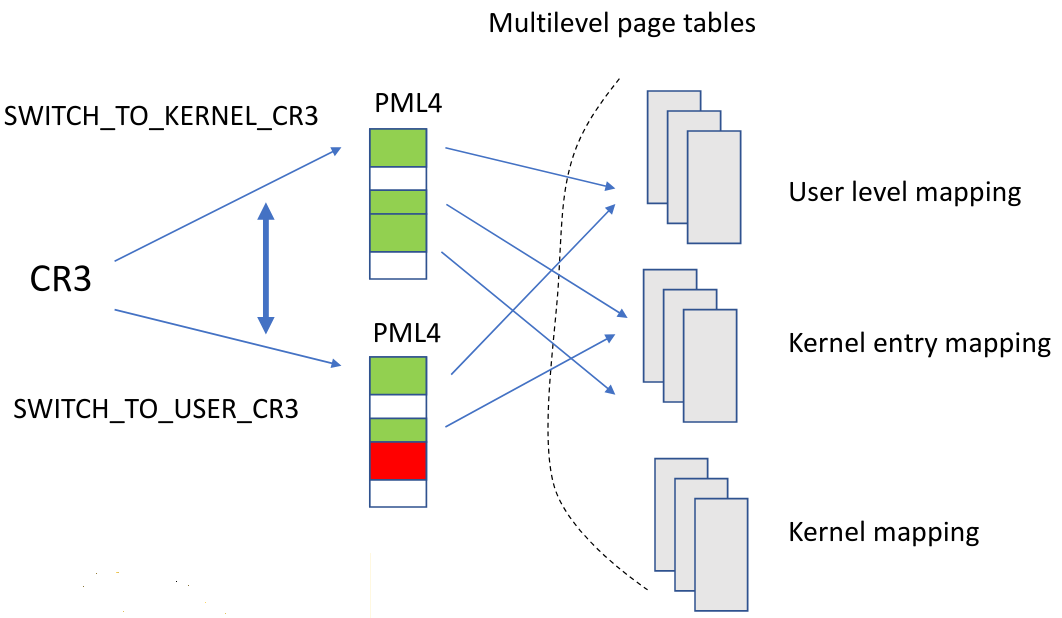
\includegraphics[scale=0.3]{immagini/KAISER}\\\\
due pt differenti, una per quando si lavora in maniera user ed una quando si lavora in kernel mode. Quando si chiama una sys call si passa ad una zona di address space in cui sono informazioni relative solo al codice kernel level, quindi non sensibile. In modo kernel, la zona di codice cambia la PT con una replicata in cui la zona è visibile, ma siamo già in modo kernel.\\ Il costo che viene pagato in termini del cambiamento della page table è che il TLB viene flushato. Nel TLB abbiamo una entry per una intera pagina, pagherò dei cache miss ma uno per pagina e non uno per ogni accesso come accade per la cache.\\ Inoltre, questa soluzione para da una serie di altri attacchi; la patch si può disattivare usando \textsf{pti=off} a livello del kernel usando GRUB. Su Linux è anche possibile mettere le patch on/off per la singola applicazione, se magari mi accorgo di un comportamento anomalo e non per tutte quelle running
\subsection{Branch}
Le sitruzioni di salto sono un altro aspetto importante nell'esecuzione del program flow: se c'è un salto, è possibile che le istruzioni che devono entrare nel program flow provengano da diversi punti dell'address space. Quando si lavoro eseguendo in pipeline, non è possibile fillare solo quando si sa che il salto è deciso o non deciso, perché ci sarebbero stalli fino a che l'istruzione non va in commit point. I salti possibili sono riassunti in 
%immagine della tabella
\begin{itemize}
\item salti condizionali: non è noto se il salto avrà luogo o no quanto questa istruzione entra in pipeline. Il numero possibile di outcome però è 2: o si salta o no
\item non condizionali: salto sempre preso, a tempo di decode si sa già che si salta e quindi siamo in grado di acquisire le istruzioni per fillare la pipe 
\item call: anche qui il salto è sempre preso
\item return: anche questo always taken, ma non sappiamo dove andare. Potremmo avere molte destinazioni, in quanto questo è funaizone della stack area e sappiamo che il valore può essere aggiornato
\item salti indiretti: implementati in modo che l'istruzione è un salto, ma il target non è un offset nell'address space bensì è dove indica un puntatore, quindi ad esempio il contenuto di un registro. La soluzione è molto usata quando dobbiamo realizzare dei function pointers
\end{itemize}
Quindi, eccetto i casi "più semplici" in cui si decide quando saltare a decode time, gli scenari sono più complessi perché bisognerebbe decidere dove saltare a commit time.\\ Esiste quindi nei processori il concetto di branch prediction: quindi, il processore ha osservato determinate istruzioni nella pipeline, e quindi se queste vengono riossservate si sa cosa fare quando la rivediamo (ad esempio se il salto è avvenuto o no).\\ Le architetture nei processori consentono di fare cose più complesse: quando lavoriamo in un processore pipeline super-scalare abbiamo un dynamic predictor che usa una Branch History Table o Branc-Prediction Buffer.\\ Ogni tabella ha una entry in cui viene indicato se saltare o no, la tabella è indicizzata dal program counter e quindi se passa una determinata istruzione viene registrato nella tabella se si è saltato o no. Se questa ripassa, si verifica col PC se c'è matching e se è così, in base al fatto che si salti o no, si decide quali istruzione caricare in pipeline.\\ Ovviamente, il salto può non avvenire, quindi poi bisogna flushare la pipeline se a commit time l'istruzione non salta. Siamo ancora in un contesto in cui le istruzioni lasciano tracce e sono problematici dal punto di vista della sicurezza.\\ Questa è una implementazione basica, inoltre nella tabella si mantengono solo alcuni dei bit che caratterizzano l'indirizzo contenuto nel PC: questo può far si che abbiamo un errore se prediciamo qualcosa che non si manifesterà, quindi il bit è 1 quando doveva essere 0 o viceversa, ma è anche possibile che nell'address space ci sia un'altra istruzione che ha la parte registrata nella tabella identica rispetto ad un altra istruzione che è quella effettivamente registrata e quindi abbiamo un altro tipo di errore. Errore = carico in pipeline determinate cose e quindi side effects
\subsubsection{Multiple bits predictors}
Una variante a due bit per un branch predictor ci dice che se una istruzione ha un certo indirizzo i, non registriamo un solo bit nella tabella bensì 2 bit, co cui possiamo discriminare 4 stadi possibili: 2 possono essere associati all'idea di saltare e due a quella di non saltare.\\ Possiamo quindi avere diversi outcome, ma se la macchina a stati è a 4 stati possiamo tenere traccia di più eventi possibili. Ad esempio, l'istruzione è passata ed è saltata, ripassando si salta. Se il salto non avviene, possiamo andare in un altro stato in cui viene detto che precedentemente è stato sbagliato il salto, ma si continua comunque a saltare.\\ Questo avviene ad esempio nei nested loop: c'è una volta in cui non si salta, ma le altre volte si salta sempre. Se ci fosse una macchina salta/non salta, l'ultima volta non salto e non posso ricordarmi che non ho saltato prima. Avrei quindi una serie di squash della pipeline.
\begin{lstlisting}
	mov $0, %ecx
\end{lstlisting}
%slides per codice e immagine
Non è l'unico modo per essere efficaci nel momento in cui abbiamo dei loop nel codice: il saltare o non saltare può essere condizionato da cosa è accaduto prima. La macchina a stati sopra è riferita ad una singola istruzione, ma le cose dipendono dal passata di più istruzioni
\subsubsection{}
Se sbagliamo, su una architettura superscalare e pipeline buttiamo decine di istruzioni magari pronte al commit, quindi è necessario andare oltre al predittore per le singole istruzioni, i due predittori che estendono il singolo sono
\begin{itemize}
\item correlato a due livelli
\item tournament predictor
\end{itemize}
Un esempio generale per considerare istruzioni di salto multiple può essere il seguente:
\begin{lstlisting}
if (aa == VAL)
	aa = 0;
if (bb == VAL)
	bb = 0;
if (aa != bb){
	// do the work
}
\end{lstlisting}
\paragraph{Predittore correlato(m,n) a due livelli:}L'idea è che c'è una importante correlazione nel flusso di esecuzione.\\ Su architetture Intel, manteniamo per ogni flusso di esecuzione un registro di esecuzione che ci dice dati gli ultimi n salti se è avvenuto o meno il salto. Nella pipeline c'è quindi una maschera che registra se è avvenuto o no il salto, la maschera può essere fatta comunque da istruzioni che possono essere committed oppure speculari, quindi una zona più recente sarà committed ed una non committed. Se la storia è fatta da due bit, possiamo discriminare 4 valori differenti, collegandoli alla history sono flussi di esecuzione completamente differenti, quindi per ciascuna di queste possibilità associamo uno specifico predittore a ciasuna combinazione dei 2 bit. I predittori indicano per l'istruzione, dato cosa è accaduto nel passato per i salti, considera cosa dice quel predittore. In generale quindi, i predittori sono tipicamente marcati con la notazione di (m,n) dove m sono gli elementi (i branch passati) mantenuti nella history ed n i bit mantenuti da ogni predittore.
\paragraph{Tournament predictor:}il predittore tiene conto del fatto che una istruzione di salto, a seconda di come è scritto il programma ha senso farlo in funzione di quali sono le istruzioni passate in pipeline prima di questa. Non è detto che il predittore correlato sia sempre il migliore, perché per la singola istruzione la storia globale può essere una penalità in base alla struttura del codice.\\ Questo predittore mantiene per ogni istruzione le informazioni di un (m,n) ed anche 2 bit per avere 4 stati:
\begin{enumerate}
\item quando si predice per una istruzione di interesse, conviene guardare tutte le cose
\item quando passa una istruzione, non guardare la history bensì solo un predittore locale
\item %slides
\end{enumerate}
Quindi, vengono messe in competizione la visione locale e quella globale. Se il flusso di esecuzione non ha molti errori, avremo una stabilizzazione che mostra "chi vince nella sfida"
\subsubsection{Salti indiretti}
Il salto indiretto è strano: se l'istruzione deve saltare, questo è funzione del risultato delle istruzioni precedenti, ovvero di cosa queste hanno scritto nei registri, che verranno usati per saltare. Quindi, il valore di tali registri può variare sempre nel tempo, quindi la predizione è più complessa ed i side effects generati sono di più.\\ L'idea è di mantenere nella stessa architettura una cache in cui vengono mantenute infroamzioni a cui associamo oltre all'indrizzo del branch anche il pre-fetched target, possiamo ache inserire dei bit per indicare quanti errori ci sono stati.\\ Nel momenti in cui c'è cache miss, non si può prelevare il salto, altrimenti viene presa; una delle istruzioni più interessanti di questo tipo in x86 è \textsf{jump [register]}, interessante per implementare function pointers etc...
%metti immagine
Quando abbiamo un errore in predizione perdiamo performance, ed inoltre ci sono problemi di sicurezza da considerare
\subsection{Attacchi spectre}
Attacchi che ancora sono in vigore, si sta studiando come introdurre delle patch a livello hardware per poter bypassare spectre con però dei costi prestazionali importanti, ad esempio disconnettere la branch prediction dinamica (forse??). Il problema è che i dati vanno avanti, ad esempio in meltdown i dati vanno in cache e cambiano lo stato micro-architetturale.\\ In spectre accade la seguente cosa: il processore ha il branch predictor, se lo caratterizziamo come componente di più ampio livello abbiamo una fase di learning e da quello il predittore decide cosa fare la prossima volta. Ma cosa fare può essere sbagliato: insegno al processore cosa fare volutamente errata, per poi passare ad un flusso dove le cose imparate non sono più valide e che quindi viene gestito male.
\subsubsection{Spectre v1}
Abbiamo un if che testa un condizione su un certo valore X, che può essere un indice usato all'interno di un array. Poi, si può scendere in un codice per cui si accede ad un array A e si usa B[X] shiftato a destra di 12, ovvero per indicizzare ogni volta 4096 byte e quindi una pagina.\\ Accediamo quindi ad A per un byte, identifichiamo il byte con B[X] ed idealmente abbiamo 256 possibilità che possono essere 256 pagine come visto in meltdown.\\ X è un indice di un'altra zona di dati, B può essere un'altra zona di memoria: sto caricando un'altra zona di informazioni spiazzandomi con X, carico il codice e lo uso per indicizzarmi con A. Quindi la posizione è in funzione di dove è B, ma anche di quanto è X: quindi, se mi sposto in una zona kernel space, funziona ancora se il branch predictor sbaglia la predizione perché è stato "allenato" così. Non abbiamo nemmeno seg fault perché è il branch predictor a fare il salto che è errato e quindi le istruzioni non vanno nemmeno in commit. Quindi, sullo stesso flusso di esecuzione possiamo fare inspection sull'array di probing A per vedere il valore he aveva B[X]. Lo spectre v1 è orientato alla problematica del branch prediction di salti condizionali.\\ Possono capitare anche cose più complesse: per come stiamo usando ora spectre, leggiamo informazioni livello kernel senza andare in seg fault, quindi il processore deve essere tale per cui l'istruzione passa comunque come offending, ma se è patchata lato hardware viene bypassata.\\ Il problema è che non basta aver risolto meltdown: quando viene eseguito del sotfware in una architettura convenzionale accade che viene chimata una syscall ad un certo punto. Quando il  kernel parte, avrà delle informazioni nei registri di processore per sapere cosa fare. Potrei aver scritto dei valori nel registro che viene usato in un check per cui si fanno determinate cose in base al valore, quindi il salto del kernel è impattato da tale valore e di conseguenza anche cosa la branch prediction fa. \\ Quindi, stabilito cosa deve avvenire quando si salta, si cambia il valore e questo permette di far eseguire al kernel speculativamente qualsiasi blocco di codice. Supponiamo di chiamare una syscall: a livello kernel c'è una tabella fatta di function pointers, ho passato tramite il registro quale valore della tabella considerare. Possiamo passare al branch un valore che è oltre la tabella, viene eseguito il salto perché il branch perdictor non sa che non deve andare oltre. Quindi, il codice del kernel si muove in funzione di cosa passa l'utente, ma così l'utente può passare parametri che alterano la branch prediction per poi attaccare. Quindi, la patch per meltdown è già stata bypassata, è stato necessario riscrivere il codice del kernel con patch per quanto riguarda il valore osservato livello kernel rispetto a quello passato dallo user, ad esempio marcando alcuni bit e tagliando il valore passato in modo che si rimane in zone incluse nella tabella.
\subsubsection{Spectre v2}
Con spectre si portano avanti anche attacchi di questo tipo: abbiamo il processore e gli hyperthread, ma il branch predictor sta nel "motore", non viene esposto a livello ISA. Il core è visibile da flussi differenti, nell'istante di tempo t abbiamo un programma P sul core, menre a t' possiamo avere P' in esecuzione: la branch prediction sta nel core, quindi P può eseguire una serie di istruzioni può dare input al branch predictor per comportarsi in un certo modo, quando c'è context swtich e cambia il programma, possiamo sfruttare il branch predictor allenato, la predizione sarà sbagliata ma abbiamo side effect sul secondo contesto che è osservabile dal primo.
%immagine con lo smile
lo scenario è che l'attaccante ha costruito il flusso di esecuzione per avere l'istruzione di salto indiretto nello stesso indirizzo dell'address space rispetto a quello della vittima, quindi quando si salta, si va in istruzioni macchine dette \textbf{gadget}, ovvero delle istruzioni che possono essere utili all'attaccante in quanto vengono creati dei side effect, ad esempio se cambio qualcosa in cache e questa è accessibile all'attaccante, il cambio è visibile.\\ Il concetto di sfruttare un gadget sulla predizione è importante per la return oriented programming, dove vengono sfruttati i gadget.\\ Ovviamente, il miss training va fatto sullo stesso CPU core della vittima, mentre il probing della cache può avvenire anche su core diversi %slides
\subsubsection{Come bypassare spectre v2}
Per salti diretti, l'unica cosa che il software può fare è ridurre il valore che viene passato nei registri per accedere alla memoria. Per quelli indiretti la patch è la \textbf{retpoline}, ovvero un trampolino basato su istruzione di ritorno. Supponiamo di dover lavorare con del software tale per cui quando il software esegue serve fare un salto indiretto queso non viene esguito, bensì il sotfware effettivo per arrivare alla destinazione viene usato un trampolino, quindi varie istruzioni in più. I trampolini sono basati sull'istruzione di ret, la soluzione vale per qualunque architettura. I passi eseguiti sono i seguenti:
\begin{enumerate}
\item viene salvato il traget dove saltare nello stack
\item si esegue una call di un pezzo di codice che rimuove il valore di ritorno del PC
\item il pezzo di codice che implementa il trampolino si trova il target dove saltare, quindi si passa tramite ret il controllo 
\item quindi il chiamato non ha un ritorno e quindi le istruzioni sottostanti sono un busy loop dummy. Quindi se viene cambiato lo stato della branch prediction
\end{enumerate}
%codice x86 di esempio
la \textsf{lea} carica l'indirizzo effettivo, viene fatto con questa istruzione perché questa non ha side effect sul processore, eliminando gli 8 byte che rappresentano il punto di ritorno della chiamata.\\ 
\subsubsection{esempio: codice per spectre}
Nel codice, viene fatto un controllo per capire quanti cicli di CPU sono necessari per un cache hit e quanti per un cache miss. Il tempo non è comunque perfetto, perché il sistema è pur sempre time sharing e quindi fra due timer possono essere successe varie cose.\\ La secret area è una pagina che metto nell'address space per potermi poi spiazzare con x ed andare nel kernel space.
\subsection{Loop unrolling}
Il problema della branch prediction è comunque legato al fatto che vogliamo cercare di saltare prima ed inoltre ridurre il numero di branches presenti in un flusso di esecuzione: se c'è un if then else non è possibile ridurlo, ma ad esempio possiamo avere un salto condizionale dalla prima istruzione all'ultima (ciclo) e vogliamo ridurre gli impatti prestazionali da un punto di vista dei salti. Il problema è che andiamo a controllare l'esecuzione del codice e quindi paghiamo altre isutrzioni macchina come overhead, per ridurre il numero di tali istruzioni viene usata tipicamente la tenica del loop unrolling: se devo girare n volte su un ciclo, scelgo di usarne $\frac{n}{2}$ o $\frac{n}{4}$ ciclo, ovvero faccio fare fare il doppio o il quadruplo delle attività al ciclo
%esempio delle slides
l'unrolling si può sviluppare sia a mano, ma non è buono perché stiamo scrivendo più linee di codice e quindi aumentando la probabilità di bug in quanto si lavorano in zone di memoria differenti. È anche possibile fare l'unloop in automatico, usando un tool di compilazione come gcc dicendo, prima di compilare una zona di codice, una opzione di compilazione \textsf{\#pragma GCC optimze ("unroll loops")}. Se facciamo l'unroll del loop, il ciclo viene esegubito un numero minore di volte nell'esegubile, ma deve eseguire più attività e quindi bisogna usare più registri e magari usare più linee di cache, quindi ci può essere un più ampio impatto sull'architettura.\\ Ci sono una serie di effetti collaterali di cui tenere conto, osservabili analizzando il codice esegubile, guardando magari nell'ELF dove è stato implementato l'unroll per verficare il fattore di unroll.
\section{Aspetti esterni al processore in una architettura IT}
Cerchiamo di capire quali sono gli impatti degli altri componenti nelle architetture IT. Siamo in uno scenario in cui abbiamo il problema del power wall: non possiamo aumentare la freqeunza dei clock più di un tot perché avremo un power cosumption tale per cui non avremmo più bilancio di calore nel chip.\\ Di fatti, il consumo di potenza cresce secondo la legge $VxVxF$ e per cui non si riresce ad andare sotto i 130W.\\ La legge di Moore dice che si possono aggiungere transistor nella CPU per poter aumentare la potenza, ma ora non è più possibile: quindi, invece di avere un solo processore, ce ne sono di più. Nell'architettura non ci sono poi solo i processori, ma anche le memorie.
\subsection{Multi processori}
% metti le due immagini diverse
Su un multi-processore simmetrico ci sono tanti oggetti simili che possono processare un flusso di programma, vedono tutti la stessa memoria, ma hanno anche delle cache private affinché i dati siano più vicini al processore.\\ Il problema è che se il dato è lo stesso e viene avvicinato ai diversi processori, questo viene replicato e c'è un problema globale nell'interazione fra processore e memoria.\\ Ora c'è il chip multi-processor, in cui ogni chip ha più di una CPU, i processori hanno delle L1 private e magari delle L2 condivise: questo è un modo con cui il vendor permette di accorpare le risorse del chipset ripsetto al caso precedente.\\ Infine abbiamo anche il symmetric multi-threading, perché se il core va molto veloce possiamo portare più di un flusso di esecuzione con gli hyperthread. Resta il problema dell'architettura di memoria per quanto riguarda la cache privata.\\ Questo tipo di chipset ha fatto si che venisse scalata in verticale anche la capacità della memoria: le attività che portano sulla memoria fanno traffico su un unica strada e questo ha portato alla creazione dell'achitettura NUMA
\subsection{Architettura NUMA}
La memoria è composta da vari slot e ciascuno ha una via principale per portare dati verso il processore. Inoltre, ogni processore può leggere dati dagli slot non vicini a lui, ma deve farlo tramite una via esterna alla sua. SUpponiamo che il core 1 debba usare solo pagine della zona di memoria a lui vicine, allora le due zone di memoria toccate sono separate e riusciamo a raddoppiare la capacità computazionale della memoria.\\ Il problema è quando vanno toccate zone di memoria non direttamente: servono strutture di itnerconnessione ed inoltre bisogna bloccare la strada per quel nodo NUMA da parte del core ricevente.\\ Lavorando in una architettura NUMA, i dati numerici ci dicono orientativamente che si aspetta dai 50 ai 200 cicli di clock per ricevere dei dati dalla memoria se si accede ad una zona vicina, altrimenti si va sui 200\%300 cicli. Si parla di sistemi scarichi, quindi aumentano parecchio se le vie sono busy per via del carico sul sistema.
\subsection{Coerenza delle cache}
Le attività basiche che caratterizzano l'hardware riguardano quello che avviene nella zona di cache: questa non è visibile nell'ISA, non è possibile toccare direttamente la cache col software per cui non si ha in maniera esplicita la possibilità di governarla.\\ C'è il problema della coerenza delle cache: la cache è un sistema di replicazione, quindi astraendo la struttura interna abbiamo un insieme di slot messi a disposizione per mantenere dati. Il dato D può essere registrato in due slot diversi, quindi quale replica si usa se qualcuno chiede di leggere un dato? Ancora peggio se avviene una scrittura sul dato: si aggiorna una sola replica o entrambe? Altra cosa interessante è che quando si parla di coerenza della cache si parla solo dell'oggetto hardware cache, ma nella CPU avvengono diverse cose (ooo, speculation etc...), ad esempio le scritture vengono fatte sullo store buffer e vengono poi portate in memoria e questo problema riguarda la memory consistency.
\subsubsection{Definizione della coerenza}
La coerenza nell'architettura di cache è definita in base a 3 proprietà:
\begin{itemize}
\item stiamo leggendo da una locazione di memoria X, precedentemente scritta dallo stesso processore ritorna l'utlimo valore scritto se nessun altro processore ha fatto nulla su quella locazione. \textbf{Causalità del program flow.}
\item {Avoidance of staleness}: se leggo da X e la lettura segue una scrittura su X da un altro processore, il valore letto è quello che è stato scritto dal processore se le due operazioni sono separate da un certo intervallo temporale
\item Tutte le scritture su X da tutti i processori sono serializzate, quindi non si possono vedere le write dai diversi processori in ordine diverso. Quindi viene gestito un ordine in modo che i dati vengano acceduti col valore corretto dai diversi processori quando c'è un update; non ci sono buffer dove vengono mantenute le cose e non vengono rese effettive (come accade ad esempio nello store buffer)
\end{itemize}
\subsubsection{Cache write through e write back con le consistenze}
Cosa accade, rispetto alla memoria, quando viene scritto un dato. Vediamo se le cose fatte da un single core basta anche per un multi-core. I due processori hanno due cache e c'è poi la memoria, vediamo la tecnica del write through, per cui il valore scritto in locale viene anche propagato sulla memoria. Se ci muoviamo con più componenti associate a processori differenti, possiamo avere che: $CPU_0$ legge X e carica 0 in cache, fa lo stesso $CPU_1$. Poi, $CPU_0$ scrive 1 su X e propaga la scrittura, ma quando $CPU_1$ legge X dalla cache legge 0 e la distanza fra le due operazioni può essere aribraria, stiamo violando il requisito 1.\\ Se usassimo write back: $CPU_0$ legge X e carica 0, $CPU_1$ legge X e carica 0. Poi $CPU_1$ scrive 1 e la scrittura non viene propagata, poi $CPU_1$ scrive 2 su X. Quindi abbiamo due valori aggiornati, uno in memoria, se $CPU_1$ fa il write back della linea in cui c'è X e poi successivamente lo fa anche $CPU_0$, il valore 2 viene sovrascritto e quindi siamo in grado di invertire l'effetto dell'update sui dati indipendentemente dalla distanza temporale fra gli update.
\subsection{Procolli di consistenza}
Le cache, oltre a mantenere i dati eseguono anche dei protocolli, quindi la logica di controllo nella cache è più articolata della letture/scrittura cache. Sono implementati a livello firmware, ed hanno 
\begin{itemize}
\item una serie di transazioni che sono supportabili fra diversi componenti hardware
\item lo stati in cui può stare un blocco di cache
\item un insieme di eventi gestiti dal controller
\item un insieme di transazioni fra stati
\end{itemize}
L'architettura può essere organizzata in maniera differente in base a diversi fattori
\begin{itemize}
\item topologia dell'interconnessione
\item primitive di comunicazione
\item gerarchia di memoria, se inclusiva o no
\item politiche di cache
\end{itemize}
i protocolli possono poi migliorare diverse performance
\begin{itemize}
\item latenza della singola transazione
\item throughput 
\item overhead dello spazio dovuto ai bit di gestione, che toglie spazio alla cache effettiva
\end{itemize}
Le famiglie classiche di protocolli sono due, che risolvono il problema di quando aggiornare le repliche nelle altre cache 
\begin{itemize}
\item invalidate protocols: quando un core scrive un blocco, tutte le altre copie diventano invalide, questo implica che si evitano le situazioni descritte prima. Solo il writer ha la possibilità di accedere alla copia aggiornata. Si incrementa la latenza ma si riduce la banda utilizzata, però chi vuole il dato non lo ha vicino nei componenti dell'architettura di caching
\item update protocols: quando avviene una scrittura, vengono aggiornate tutte le altre copie. Si pagano però costi importanti per l'aggiornamento dei dati: ogni copia del blocco è sempre aggiornata alla copia coerente. Abbiamo il trade-off fra banda e latenza: ognuno prende la copia dal vicino ma si paga sulla banda
\end{itemize}
I primi sono quelli usati in architetture moderne, per cui ci focalizziamo su quelli per capire come avviene l'invalidazione
\subsubsection{Snooping cache}
Come lavorano effettivamente i vari componenti dell'architettura hardware per implmenetare l'invalidate protocol: tutti i componenti sono conessi fra loro tramite un mezzo broadcast, anche detto rete, quindi tutte le cache possono parlare con tutte. È un modo semplice per poter prendere il mezzo, comunicare a tutti ad esempio un cambio di stato per far si che tutti lo cambino. C'è la serializzazione di tutte le transazioni: quando la CPU va sull'interfaccia verso la cache, l'interazione deve usare il broadcast medium, ma se non è necessario che ci sia la transazione distribuita non si parla. Se quando si manda l'interazione verso l'architettura di cache e questo genera un evento tale per cui qualcun altro deve parlare c'è la serializzazione, quindi nella time line i cambi di stato avvengono quando quello precedente è completato. I componenti di caching sono connessi a dei controller che è in grado di capire i messaggi di broadcast per poter effettuare i cambi di stato.
%immagine dalle slides.
\\ Le azioni trattano le singole linee di cache, per cui quando qualcuno parla lo fa per quella linea di cache.
\subsubsection{MSI protocol}
Per ogni operazione, attribuiamo un timbro alla liena di cache:
\begin{itemize}
\item modified
\item invalid
\item shared: la versione più è condivisa fra vari componenti.
\end{itemize}
Quando qualcuno deve fare una scrittura su una linea di cache viene inviato un messaggio in broadcast tale per cui chiunque altro ha la linea in uno stato non invalid la marca come invalid.\\ La transazione di lettura prende l'ultima versione aggiornata dalla memoria in una cache write through, possiamo prendere l'ultimo valore aggirnato 
da un altro componente in caso di write back. Dobbiamo tenere traccia dello stato del blocco, se questo è modificato oppure shared, questo è atomico e viene fatto da tutti in ogni intervallo di tempo.
\subsubsection{Protocollo MESI}
Gli stati di una linea di cache possono essere 4
\begin{itemize}
\item Invalid
\item Modified
\item Shared
\item Exclusive: il componente di cache indica che fa una gestione esclusiva di quella linea di cache. Ovvero quel componente può fare ciò che vuole senza dover dire a nessuno che ha scritto la linea. Quindi, questo può avvenire senza interazioni con nessuno: se un program flow tocca un dato per aggiornarlo di continuo, non è necessario comunicare ad altri componenti che questo è accaduto.
\end{itemize}
Quindi, non è vero che qualcuno legga qualcosa di vecchio, perché questo è vero solo se qualcuno passa ad exclusive e rende invalide le altre copie.
%immagine dell'automa
\textbf{esempio: transazioni in risposta a letture locali}\\
se lo stato è M, E o S non succede nulla. (slides)
\textbf{esempio: transazioni in risposta a scritture locali}\\
\begin{itemize}
\item se lo stato è M non ci sono transazioni
\item se lo stato è E non ci sono transazioni sul bus e si fa in M
\item se lo stato è S, la linea è in locale ma posso avere le altre copie e quindi tramite l'uso del bus genero una richiesta di read per prendere l'uso esclusivo
\item (slides)
\end{itemize}
ALTRI ESEMPI SULLE SLIDES
\subsubsection{MOESI}
Variante del MESI in cui c'è uno stato in più che è Owned, ovvero una cache line può essere Owned e la differenza rispetto ad Exclusive è che se aggiorno della linea di cache, gli altri la hanno invalida. In O è possibile che se aggiorno la linea do la copia a chi la chiede ma lo avviso che essendo l'owner potrei aggiornare la linea in futuro e che chi al riceve non può più aggiornarla; questo evita la transizione in diversi stati come avveniva prima.
\subsubsection{Implementazioni in x86}
Tipicamente, in Intel
\begin{itemize}
\item MESI
\item Cache inclusive
\item Write back
\item Cache L1 con linee a 64 byte
\end{itemize}
AMD
\begin{itemize}
\item MOESI
\item Cache esclusiva ad L3
\item Write back
\item Cache L1 con linee a 64 byte
\end{itemize}
\subsubsection{Alternativa allo snooping}
Lo snooping va bene quando la scala dell'architettura non è grande, ma se la scala cresce e si parla tutti con tutti ci sono problemi di delay.\\ Quindi, lo snooping non scala bene, per cui si risolve usando soluzioni directory-based:
\begin{itemize}
\item non c'è più il broadcast, i componenti comunicano indirettamente fra loro
\item al centro della comuniazione c'è la directory, che mantitene i metadati
\end{itemize}
Quindi, per parlare con i componenti, non è datto che debba parlare con tutti ma lo faccio solo con la directory. Inoltre, la directory serializza tutte le attività solo internamente.
\paragraph{Funzionamento della directory:}per ogni unità portata dalla RAM alla cache, vengono mantenuti dei metadati, dove indichiamo che sta mantenendo la copia del dato e se il dato è dirty. %immagine dalle slides
Possiamo quindi dire che c'è una versione aggiornata presso un componente della cache, che è in corrispondenza di chi ha il dato aggiornato (l'1 azzurrino) e quindi poi si aggiorna, se qualcuno richeide il dato, chi lo mantiene.\\ \textbf{esempio:}\\ Abbiamo un read miss per $P_0$, quindi andando dalla directory scopre chi ha la copia del dato, consegnarlo e marcare il bit pari ad 1. In questo modo, sappiamo che quando qualcuno scrive dobbiamo invalidare solo alcuni dei processori ovvero quelli che hanno il dato shared.
\subsection{Relazione fra software e performance della cache}
La scrittura del software produce un program flow che poi finisce in cache, a seconda di ciò che viene scritto. Supponiamo di avere un program flow in cui si cerca di accedere in memoria per prelevare un dato e quel dato è in una certa linea di cache. Supponiamo poi di avere un altra istruzione che vuole leggere un altra area di memoria, quindi in corrispondenza di un'altra linea di cache: abbiamo la località dei dati user space\\ Il problema è grave se giriamo con più thread o hyperthread o più processi in concorrenza che accedono in memoria: le istruzioni chiamate toccano le stesse strutture dati, le interazioni chiamate cambiano lo stato MESI delle linee di cache, quello che bisogna evitare quando si scrive codice di kernel è che i dati usati più spesso devono essere sulla stessa linea di cache in modo da diminuire gli accessi in cache.\\ Le informazioni scarsamente correlate fra loro non devono invece cadere sulla stessa linea di cache, perché se due thread vogliono scrivere su due diversi byte e questi sono nella stessa linea di cache interagiscono con il protollo MESI chiamando un maggiore numero di transazioni, sharando la linea di cache.\\ In modo che il software sia scritto bene, occorre sapere se l'area di memoria logica è allineata con la linea di cache: viene dato un pointer dalla malloc e vogliamo che i 64 byte logici che otteniamo siano allineato coi 64 byte della linea di cache così da avere un buffer cache aligned. Questo dipende dal tipo di allocatore che si usa:
\begin{itemize}
\item \textsf{posix\_memalign }
\item \textsf{aligned\_alloc }
\item \textsf{valloc }
\end{itemize}
\end{document}
